\documentclass{article}

\usepackage{graphicx}
%\usepackage{subfigure}
\usepackage{caption}
\usepackage{subcaption}

\begin{document}

\begin{figure}
    \centering
    \begin{subfigure}[b]{0.3\textwidth}
        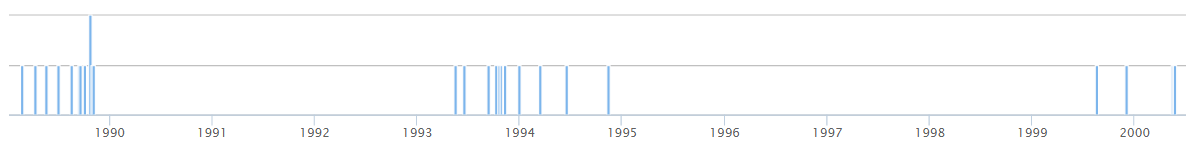
\includegraphics[width=\textwidth]{../images/rg_timeline_pm230.png}
        \caption{A gull}
        \label{fig:gull}
    \end{subfigure}%
    ~ %add desired spacing between images, e. g. ~, \quad, \qquad etc.
      %(or a blank line to force the subfigure onto a new line)
    \begin{subfigure}[b]{0.3\textwidth}
        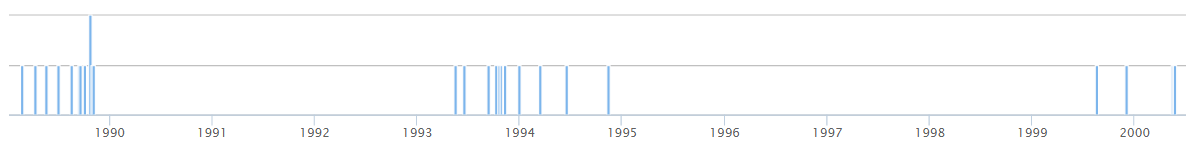
\includegraphics[width=\textwidth]{../images/rg_timeline_pm230.png}
        \caption{A tiger}
        \label{fig:tiger}
    \end{subfigure}
    ~ %add desired spacing between images, e. g. ~, \quad, \qquad etc.
      %(or a blank line to force the subfigure onto a new line)
    \begin{subfigure}[b]{0.3\textwidth}
        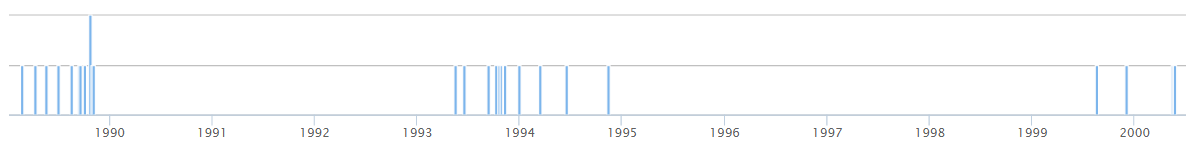
\includegraphics[width=\textwidth]{../images/rg_timeline_pm230.png}
        \caption{A mouse}
        \label{fig:mouse}
    \end{subfigure}
    \caption{Pictures of animals}\label{fig:animals}
\end{figure}

\end{document}